%======================================================================
\subsection{BW-PDM-10 --- Plan: the vault dashboard (24 Oct 2026, approved 24 Oct)}\label{sec:pdm10-plan}
%======================================================================

On 24 Oct you asked: ``is there a vault view after creating the vault? like a dashboard of everything?'' Not yet. With a
vault open, the Start page shows the vault switcher, \emph{My work} (checked out to me, waiting for review, newer in the
vault, ECOs open) and the vault's recent files. It has no overview: it gives no counts, no projects, no activity and no
word on whether iCloud is in step. You also said ``for the vault I shouldn't have files showing up in it''. That is built
today: with a vault open, the recent list keeps only files inside the vault folder
(\code{vault\_folder}/\code{in\_folder} in \file{bruceworx\_start.py}). This plan makes the vault side of the Start page
a dashboard of the whole vault. It follows the same rule: \textbf{vault items only, never local files}.

\begin{center}
\small
\begin{tabularx}{\linewidth}{@{}>{\raggedright\arraybackslash}p{3.0cm}X@{}}
\toprule
Section & What it shows (each opens the matching filtered list)\\
\midrule
Header & vault name, sync state (``up to date, read 1 min ago''), where it lives, who you are in it, its units;
  \emph{New Project\ldots}, \emph{Import Files\ldots}, \emph{Vault panel}\\
Tiles & parts, assemblies, drawings and bought items, each with a bar of WIP / in review / released / obsolete;
  drawings out of date (\eref{PDM-09}~B)\\
Projects & each project's top assembly, how much of it is released, in review or in work, and its drawing problems\\
My work & today's queues, capped at a few rows each: checked out to me, waiting for review, drawings out of date, newer in
  the vault, ECOs open\\
Changes & open ECRs and ECOs with their state and what each waits for (\file{bruceworx\_changes.py})\\
Activity & who did what and when, from the journal: check-ins, submissions, releases, rejections, ECR/ECO steps, new
  projects; grouped, 14 days by default\\
Vault health & iCloud (on this Mac, cloud only, still syncing), locks and their age, journal problems, reading time\\
Recent in this vault & the cards and table of today, vault files only\\
\bottomrule
\end{tabularx}
\end{center}
It builds on the folder vault (\eref{PDM-04}, \S\ref{sec:pdm04-plan}), review and change control (\eref{PDM-05},
\S\ref{sec:pdm05-plan}), the per-revision BOM (\eref{PDM-06}, \S\ref{sec:pdm06-plan}) and PDM-09's projects and drawing
states (\S\ref{sec:pdm09-plan}).

%----------------------------------------------------------------------
\subsubsection*{1. What the spikes showed (24 Oct)}

A generator script (\file{dashboard-plan/spike\_gen.py}) made three scratch vaults through the real engine
(\file{pdm\_folder.py}, \file{pdm\_workspace.py}). Each has 74\,\% parts, 11\,\% assemblies with BOMs, 17\,\% drawings
and 4\,\% COTS. Events are spread over 120 days with two actors, \code{bruce@mac} and \code{alex@mbp}. Each vault has
releases, ECRs, ECOs (some released), locks and work copies. A second script (\file{spike\_time.py}) timed each read the
dashboard makes, in Homebrew Python 3.12 and again inside \code{FreeCADCmd} (Python 3.11): the numbers agree within
10\,\%. Your vault \emph{Vector} was not opened.
\begin{center}
\footnotesize
\begin{tabular}{@{}lrrr@{}}
\toprule
Scratch vault & 500 items & 2\,000 items & 5\,000 items\\
\midrule
Journal events / size & 2\,312 / 0.6\,MB & 9\,249 / 2.3\,MB & 23\,134 / 5.7\,MB\\
Read and parse the journal & 3\,ms & 13\,ms & 34\,ms\\
\textbf{Open the vault (read + replay)} & \textbf{8\,ms} & \textbf{74\,ms} & \textbf{429\,ms}\\
\quad replay without the per-BOM cycle check & 5\,ms & 20\,ms & 59\,ms\\
\code{status()} / \code{missing\_objects()} & 2 / 2\,ms & 8 / 6\,ms & 19 / 16\,ms\\
\code{Workspace.my\_work()} & 2\,ms & 9\,ms & 23\,ms\\
Start page's \code{read\_vault} today (all of it) & 17\,ms & 119\,ms & 545\,ms\\
Dashboard aggregation (prototype) & 6\,ms & 100\,ms & 719\,ms\\
\quad project roll-up, memoised (all top assemblies) & 0.2\,ms & 0.7\,ms & 2\,ms\\
Peak memory of a replay & 3.6\,MB & 15\,MB & 38\,MB\\
Has anything changed? (\code{vault\_signature}) & $<$0.1\,ms & $<$0.1\,ms & $<$0.1\,ms\\
Read only the new journal lines (none new) & 0.03\,ms & 0.07\,ms & 0.11\,ms\\
Main-thread stall while a worker replays (max) & 8\,ms & 8\,ms & 16\,ms (28\,ms in FreeCAD)\\
\bottomrule
\end{tabular}
\end{center}

\paragraph{Findings.}
\begin{enumerate}[nosep]
  \item \textbf{At the size you will have for a long time, nothing stalls.} A 500-item vault reads, replays and summarises
        in about 25\,ms on the worker thread that the Start page already uses (\code{\_Loader}). The main thread never
        waited more than two of Python's 5\,ms switch intervals, even during a 0.5\,s replay. So the worker thread is enough;
        no separate process is needed.
  \item \textbf{The replay is quadratic, and BOMs cause it.} A profile of the 5\,000-item replay puts 90\,\% of its time in
        \code{pdm.Vault.set\_bom}. Each call checks the \emph{whole} BOM graph for a cycle (\code{\_cycle}) and rebuilds the
        \code{bom} map from every item. Every assembly check-in whose BOM changed records a \code{set\_bom}
        (\file{bruceworx\_bom.py}), so the cost grows with use, not only with size (theory below). The fix is small and
        lives in the engine (step~1).
  \item \textbf{My prototype's project roll-up was quadratic too.} It called \code{flattened(top)} once per top assembly.
        A memoised walk, bottom-up, does all of them in 2\,ms.
  \item \textbf{Today's \emph{My work} does not scale.} In the 500-item vault it listed 25 checked-out files, then
        \emph{every} item in review (15), then the open ECOs, all in one uncapped table (the screenshot behind
        figure~\ref{fig:pdm10-light}). ``Waiting for review'' means \emph{anything} in review: the vault has no reviewers yet.
  \item \textbf{The Start page reads the journal twice.} \code{read\_vault} opens a \code{FolderVault}, which replays it,
        then calls \code{\_read\_events()} again to count this week's releases. That is 3\,ms at 500 items and 34\,ms
        at 5\,000. The vault could keep the sorted events it already read.
  \item \textbf{A race on \file{state.json}.} \code{Workspace.statuses()} saves the hashes it computed back to
        \file{work/<actor>/.bw/state.json}. The worker thread does this with its own \code{Workspace}, loaded a moment
        earlier. A check-out on the GUI thread in that window records a new base, and the worker's save then overwrites it.
        The window is a few milliseconds, but the dashboard reads more often than today's page. Its workspace must not write
        (step~1).
  \item \textbf{Two facts the dashboard needs are not kept.} (a) A lock has a holder but no start time (\code{locks} maps
        P/N to actor), so ``oldest lock 2 days'' cannot be shown. (b) \code{missing\_objects()} uses
        \code{os.path.exists}. An object that iCloud evicted to a \file{.<name>.icloud} stand-in (macOS 13 and older) counts
        as \emph{missing}, although it is only waiting to download. On macOS 14 and later evicted files stay as dataless
        files and are handled correctly. \code{pdm\_workspace.needs\_download} already tells these cases apart.
  \item \textbf{A third of the journal is noise for a feed.} Check-outs make up 33\,\% of the events, check-ins 31\,\% and
        \code{set\_bom} 2\,\%. The feed shows check-ins, releases and changes, folds runs together, and hides check-outs
        unless asked.
\end{enumerate}

%----------------------------------------------------------------------
\subsubsection*{2. Theory}

\paragraph{The dashboard is a function of the journal.} Nothing on the page is stored for it. With $J$ the merged, sorted
journal, $W$ your work folder's \file{state.json}, $t$ the time now and $a$ your pinned actor, the page shows
\[
  D = f(J, W, t, a) = \bigl(\text{counts},\ \text{projects},\ \text{queues}_a,\ \text{changes},\ \text{activity}_{[t-\Delta,\,t]},\ \text{health}\bigr),
\]
where every part is computed from the replayed state $S = \mathrm{fold}(\mathrm{apply}, S_0, J)$. Two Macs with the same
journal show the same page, apart from \emph{My work} and the sync line. A page that disagrees with the Vault panel is
therefore a bug, not a timing issue. The header always says ``read $n$ min ago'', so a stale page shows that it is stale.

\paragraph{Cost of a replay.} With $E$ events, $N$ items, $L$ BOM lines and $S$ \code{set\_bom} events, the measured cost is
\[
  T_\text{replay} \approx \alpha E + \gamma\, S\,(N + L), \qquad \alpha \approx 2.5\,\mu\text{s},\quad \gamma \approx 80\,\text{ns},
\]
fitted on the three vaults (each constant within 20\,\% across them). The second term is the whole-graph cycle check on
every \code{set\_bom}. It is quadratic in practice, because $S$ grows with every assembly check-in. For example, a vault with
$N = 2\,000$, $L = 1\,500$ and $E = 10\,000$, after a year of $S = 1\,000$ assembly check-ins, takes 25\,ms for the first
term and 280\,ms for the second.

The fix: a journal line was checked when it was written (\code{\_record} runs strict), so a replay need not check it
again. Run the cycle check \emph{once} after the replay, at $O(N + L)$. It still catches a cycle that only appears when two
Macs' journals merge, and records it as a problem. The \code{bom} map is cached and updated per \code{set\_bom} instead of
being rebuilt. The cost becomes $T \approx \alpha E$: about 60\,ms at 23\,000 events.

\begin{figure}[!htbp]
\centering
\begin{tikzpicture}[x=0.0021cm,y=0.0105cm,font=\scriptsize]
\draw[black!30] (0,0) -- (5300,0); \draw[black!30] (0,0) -- (0,470);
\foreach \x in {0,1000,2000,3000,4000,5000} { \draw[black!30] (\x,0) -- (\x,-6); \node[below=2pt] at (\x,0) {\x}; }
\foreach \y in {0,100,200,300,400} { \draw[black!30] (0,\y) -- (-60,\y); \node[left=2pt] at (0,\y) {\y}; }
\node[below=12pt] at (2650,0) {items in the vault (events $\approx 4.6\times$)};
\node[rotate=90] at (-560,235) {ms};
\draw[bwred,thick] (500,8) -- (2000,74) -- (5000,429);
\foreach \p in {(500,8),(2000,74),(5000,429)} \fill[bwred] \p circle (1.6pt);
\draw[bwgreen,thick] (500,4.8) -- (2000,20.2) -- (5000,59);
\foreach \p in {(500,4.8),(2000,20.2),(5000,59)} \fill[bwgreen] \p circle (1.6pt);
\draw[bwblue,thick,dashed] (0,25) -- (5300,25);
\node[bwred,anchor=east] at (3500,330) {today: cycle check per BOM};
\node[bwgreen!80!black,anchor=west] at (3500,85) {one check after the replay};
\node[bwblue,anchor=west] at (5320,25) {25\,ms};
\end{tikzpicture}
\caption{Time to open a vault (read and replay the journal) against its size, measured on three scratch vaults. The red
curve is today's engine, the green one has the cycle check moved to the end. The dashed line is about one frame of
animation at 40\,Hz. Your vaults stay left of 500 items for a long time.}
\label{fig:pdm10-cost}
\end{figure}

\paragraph{Reading only what is new.} The journal files are append-only, one per actor. Keep the byte offset $o_f$ read
from each file $f$ and the sort key $k^\ast = (\mathit{at}, \mathit{actor}, \mathit{seq})$ of the last event applied. A
refresh reads only the new complete lines $N$ past $o_f$. Since the replay is a left fold over the sorted events,
\[
  \min_{e \in N} k(e) > k^\ast \ \Longrightarrow\ \mathrm{fold}(J \mathbin{+\!\!+} N) = \mathrm{fold}\bigl(N,\ \mathrm{fold}(J)\bigr),
\]
so the new events can be applied to the state already held. This holds whenever this Mac is the only writer. If any new
event sorts \emph{before} $k^\ast$, the incremental state could differ from a full replay. That happens when another Mac's
line arrives late through iCloud, or when its clock is behind. The same goes for a file that shrank or was replaced, or a
new conflict copy. In all these cases, do one full replay. The check costs 0.1\,ms when nothing is new, so the page can poll
it every few seconds while it is visible.

\paragraph{Project progress.} A project's closure is its top assembly, everything its BOM reaches (\code{explode}, the DAG
of \S\ref{sec:pdm06-plan}) and their drawings: $C(p) = \{t_p\} \cup \mathrm{reach}(t_p) \cup \mathrm{drawings}(\cdot)$.
Each item counts once, whatever its quantity, because a bolt used 40 times is one item to release. Progress is the share in
each state,
\[
  \pi_s(p) = \frac{|\{x \in C(p) : \mathrm{state}(x) = s\}|}{|C(p)|}, \qquad s \in \{\text{Released}, \text{In Review}, \text{WIP}\},
\]
drawn as one stacked bar. A memoised walk computes $\mathrm{reach}$ for every assembly bottom-up, so all projects together
cost $O(N + L)$. The spike measured 2\,ms for 385 top assemblies, against 31\,ms for 20 separate
\code{flattened()} calls. Until PDM-09 records projects (\code{create\_project}), the stand-ins are \emph{top assemblies}:
assemblies that no other assembly's BOM uses, marked ``top assembly'' rather than ``project''.

\paragraph{Folding the activity feed.} Consecutive events $e_i, e_{i+1}$ fold into one line when they have the same actor
and operation and $|\mathit{at}_{i+1} - \mathit{at}_i| \le 10$\,min: ``You checked in 6 files'', with the comment when all
six share it. The feed shows \code{checkin}, \code{submit}, \code{approve}, \code{reject}, \code{retire}, the four ECR/ECO
operations, \code{create\_item} (folded: ``created 13 items'') and \code{create\_project}. \emph{Show all} adds
\code{checkout}, \code{undo\_checkout} and \code{set\_bom}. The bars above the feed count the shown events per day.

\begin{figure}[!htbp]
\centering
\begin{tikzpicture}[>=Stealth,node distance=5mm and 6mm,
  b/.style={draw=bwblue!70,fill=bwblue!5,rounded corners=2pt,font=\scriptsize,align=center,minimum height=0.95cm,text width=2.35cm},
  g/.style={b,draw=bwgreen!80,fill=bwgreen!8},
  o/.style={b,draw=bworange!80,fill=bworange!8},
  t/.style={font=\tiny\color{bwgrey},align=center}]
\node[b] (j) {{\ttfamily journal/*.jsonl}\\{\ttfamily work/<me>/.bw/\\state.json}\\objects (iCloud)};
\node[o,right=of j] (w) {Worker thread\\signature $\rightarrow$ tail or full replay};
\node[g,right=of w] (d) {{\ttfamily vault\_\\dashboard.py}\\snapshot $D$ (a dict, $\approx$5\,kB)};
\node[b,right=of d] (p) {Start page\\header, tiles, projects, queues, feed, health};
\node[b,below=7mm of p] (v) {Vault panel / Vault tab\\filtered list, item selected};
\node[b,below=7mm of w] (l) {FreeCAD's own operations\\(vault listeners)};
\draw[->] (j) -- (w); \draw[->] (w) -- (d); \draw[->] (d) -- node[t,above] {signal} (p);
\draw[->] (p) -- node[t,right] {click a tile or row} (v);
\draw[->] (l) -- node[t,left,pos=0.4] {refresh} (w);
\node[t,above=1mm of w] {never on the GUI thread; writes nothing};
\node[t,above=1mm of d] {FreeCAD-free, tested};
\end{tikzpicture}
\caption{Where the dashboard's numbers come from. Green is the new module, orange the existing worker (\code{\_Loader})
with incremental reading added.}
\label{fig:pdm10-flow}
\end{figure}

%----------------------------------------------------------------------
\subsubsection*{3. Design}

\begin{figure}[!htbp]
\centering
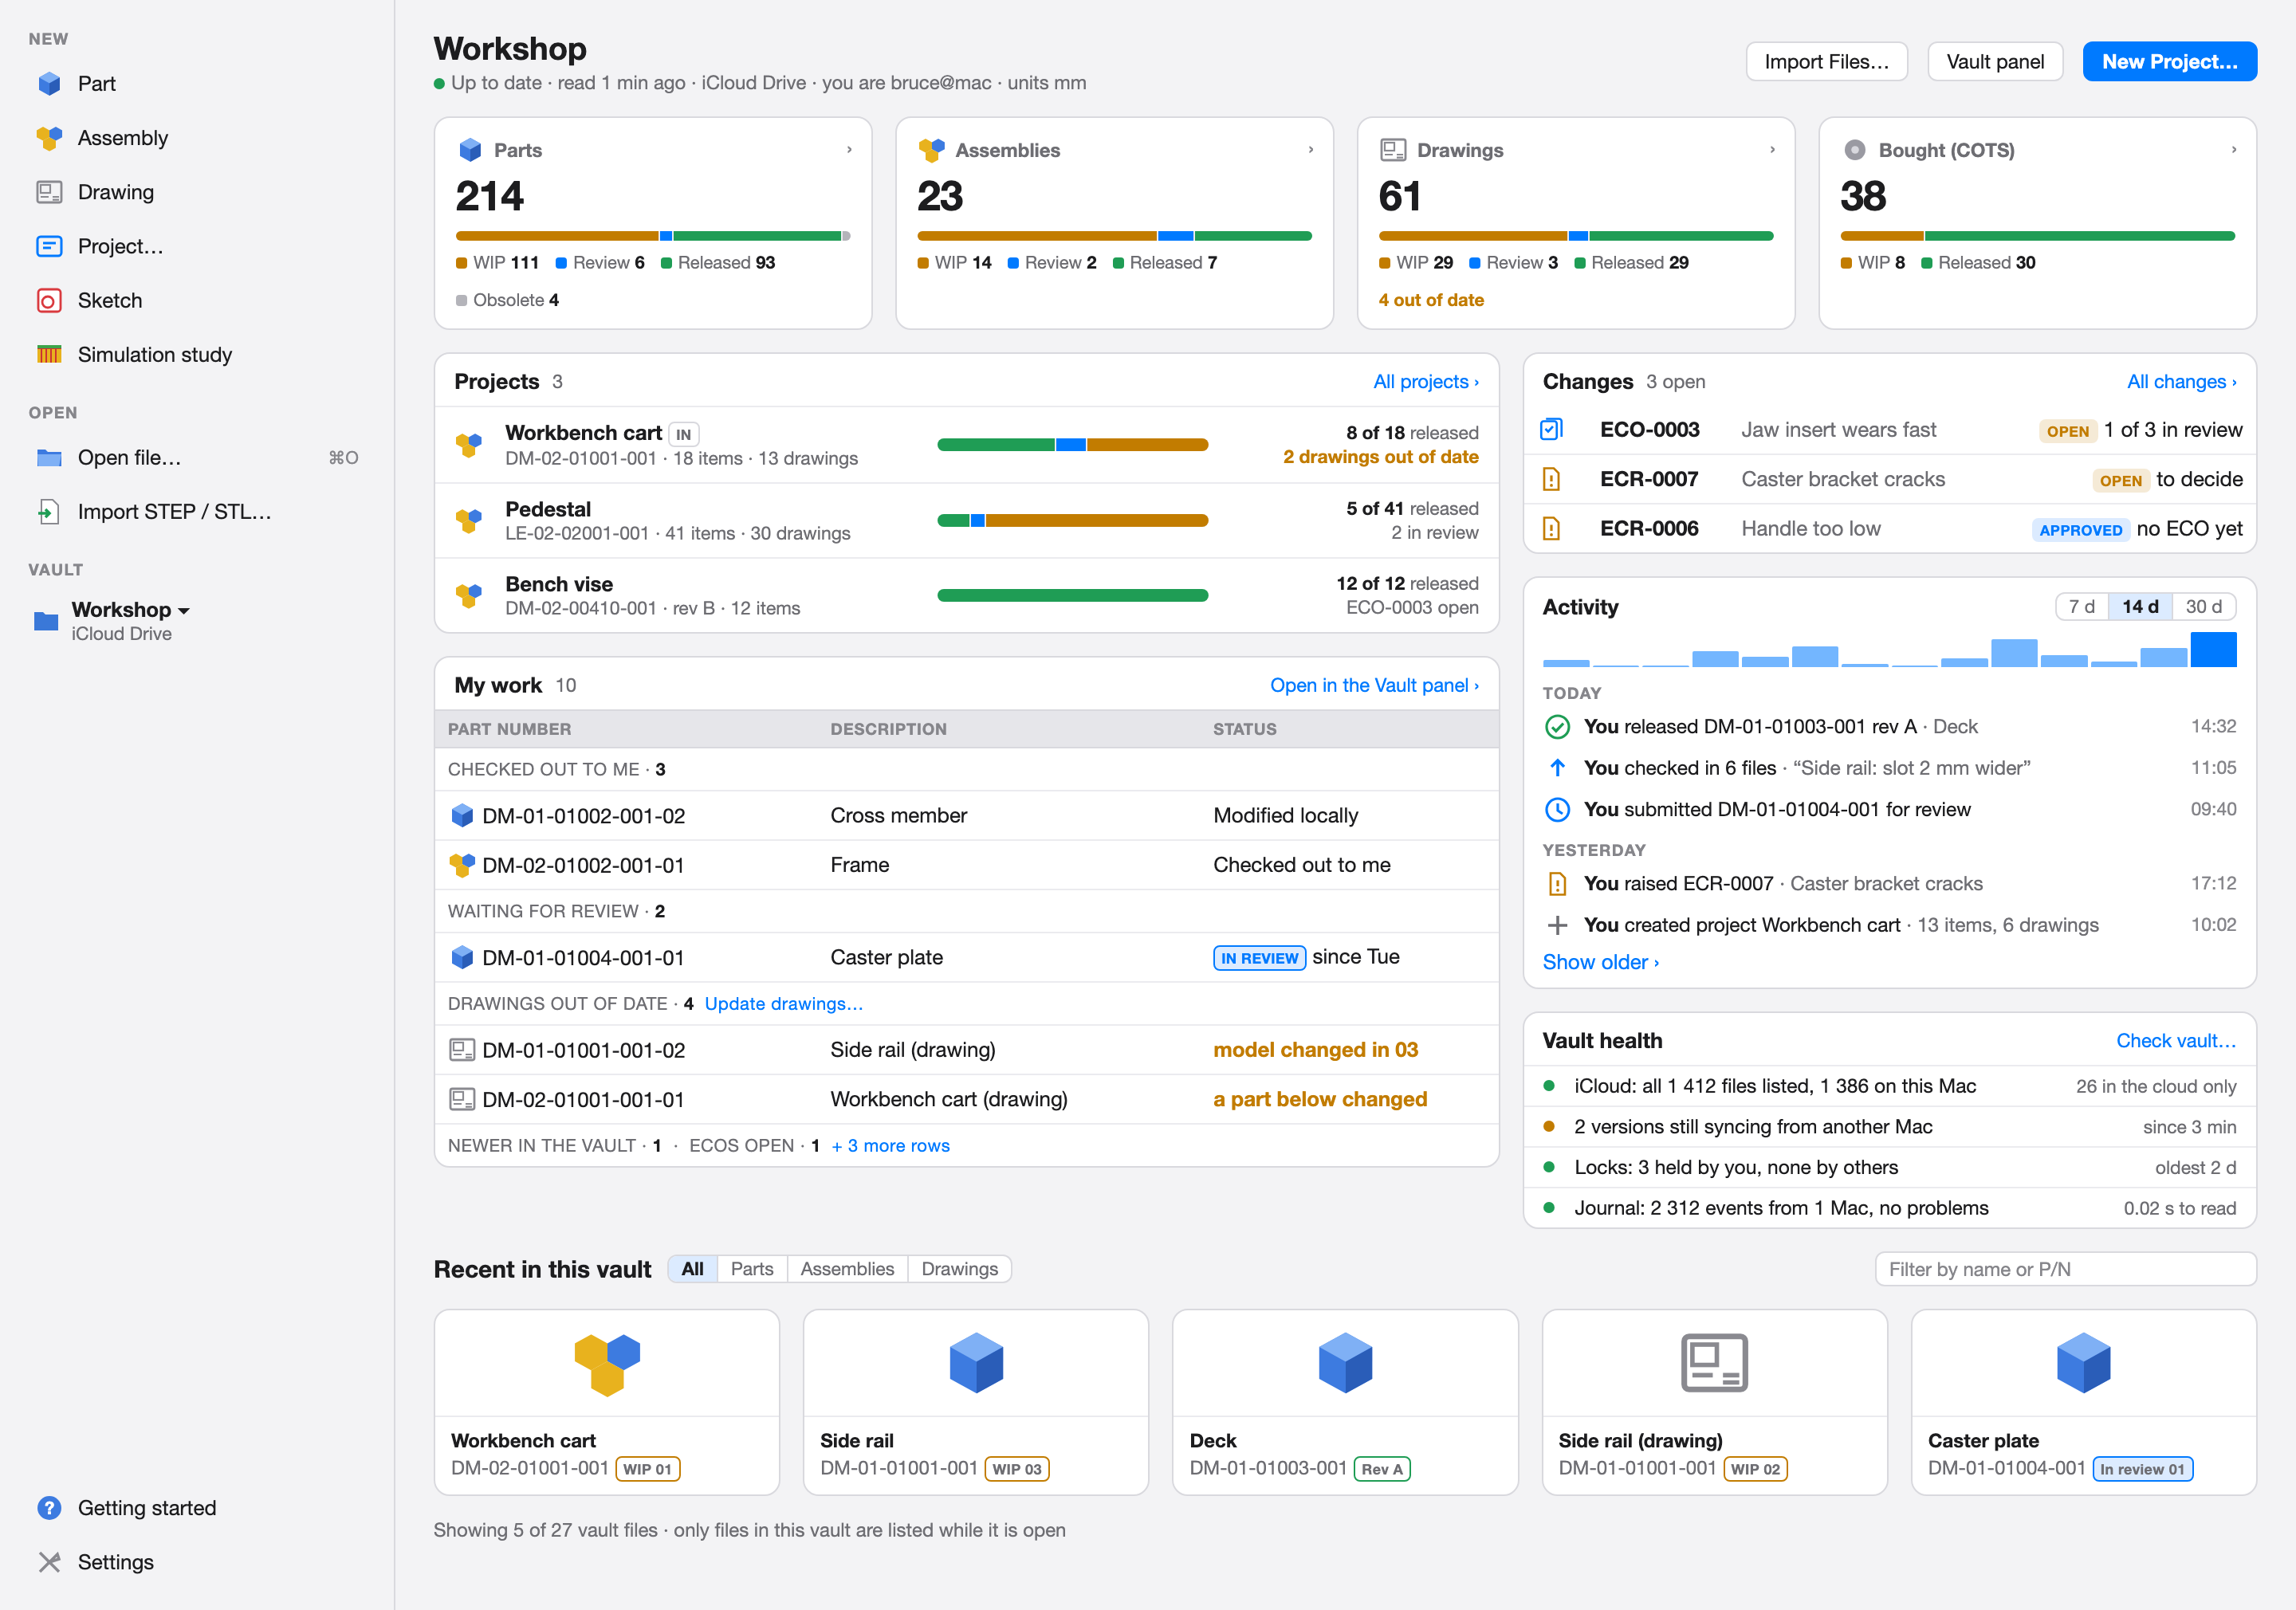
\includegraphics[width=\linewidth]{fig/pdm10_dashboard_light.png}
\caption{Mock: the Start page with a vault open is the vault's dashboard. The left column is today's, with \emph{Project\ldots}
(\eref{PDM-09}) under \emph{New}. Every tile, project, row and health line opens the matching filtered list. The sample data
is invented.}
\label{fig:pdm10-light}
\end{figure}

\begin{figure}[!htbp]
\centering
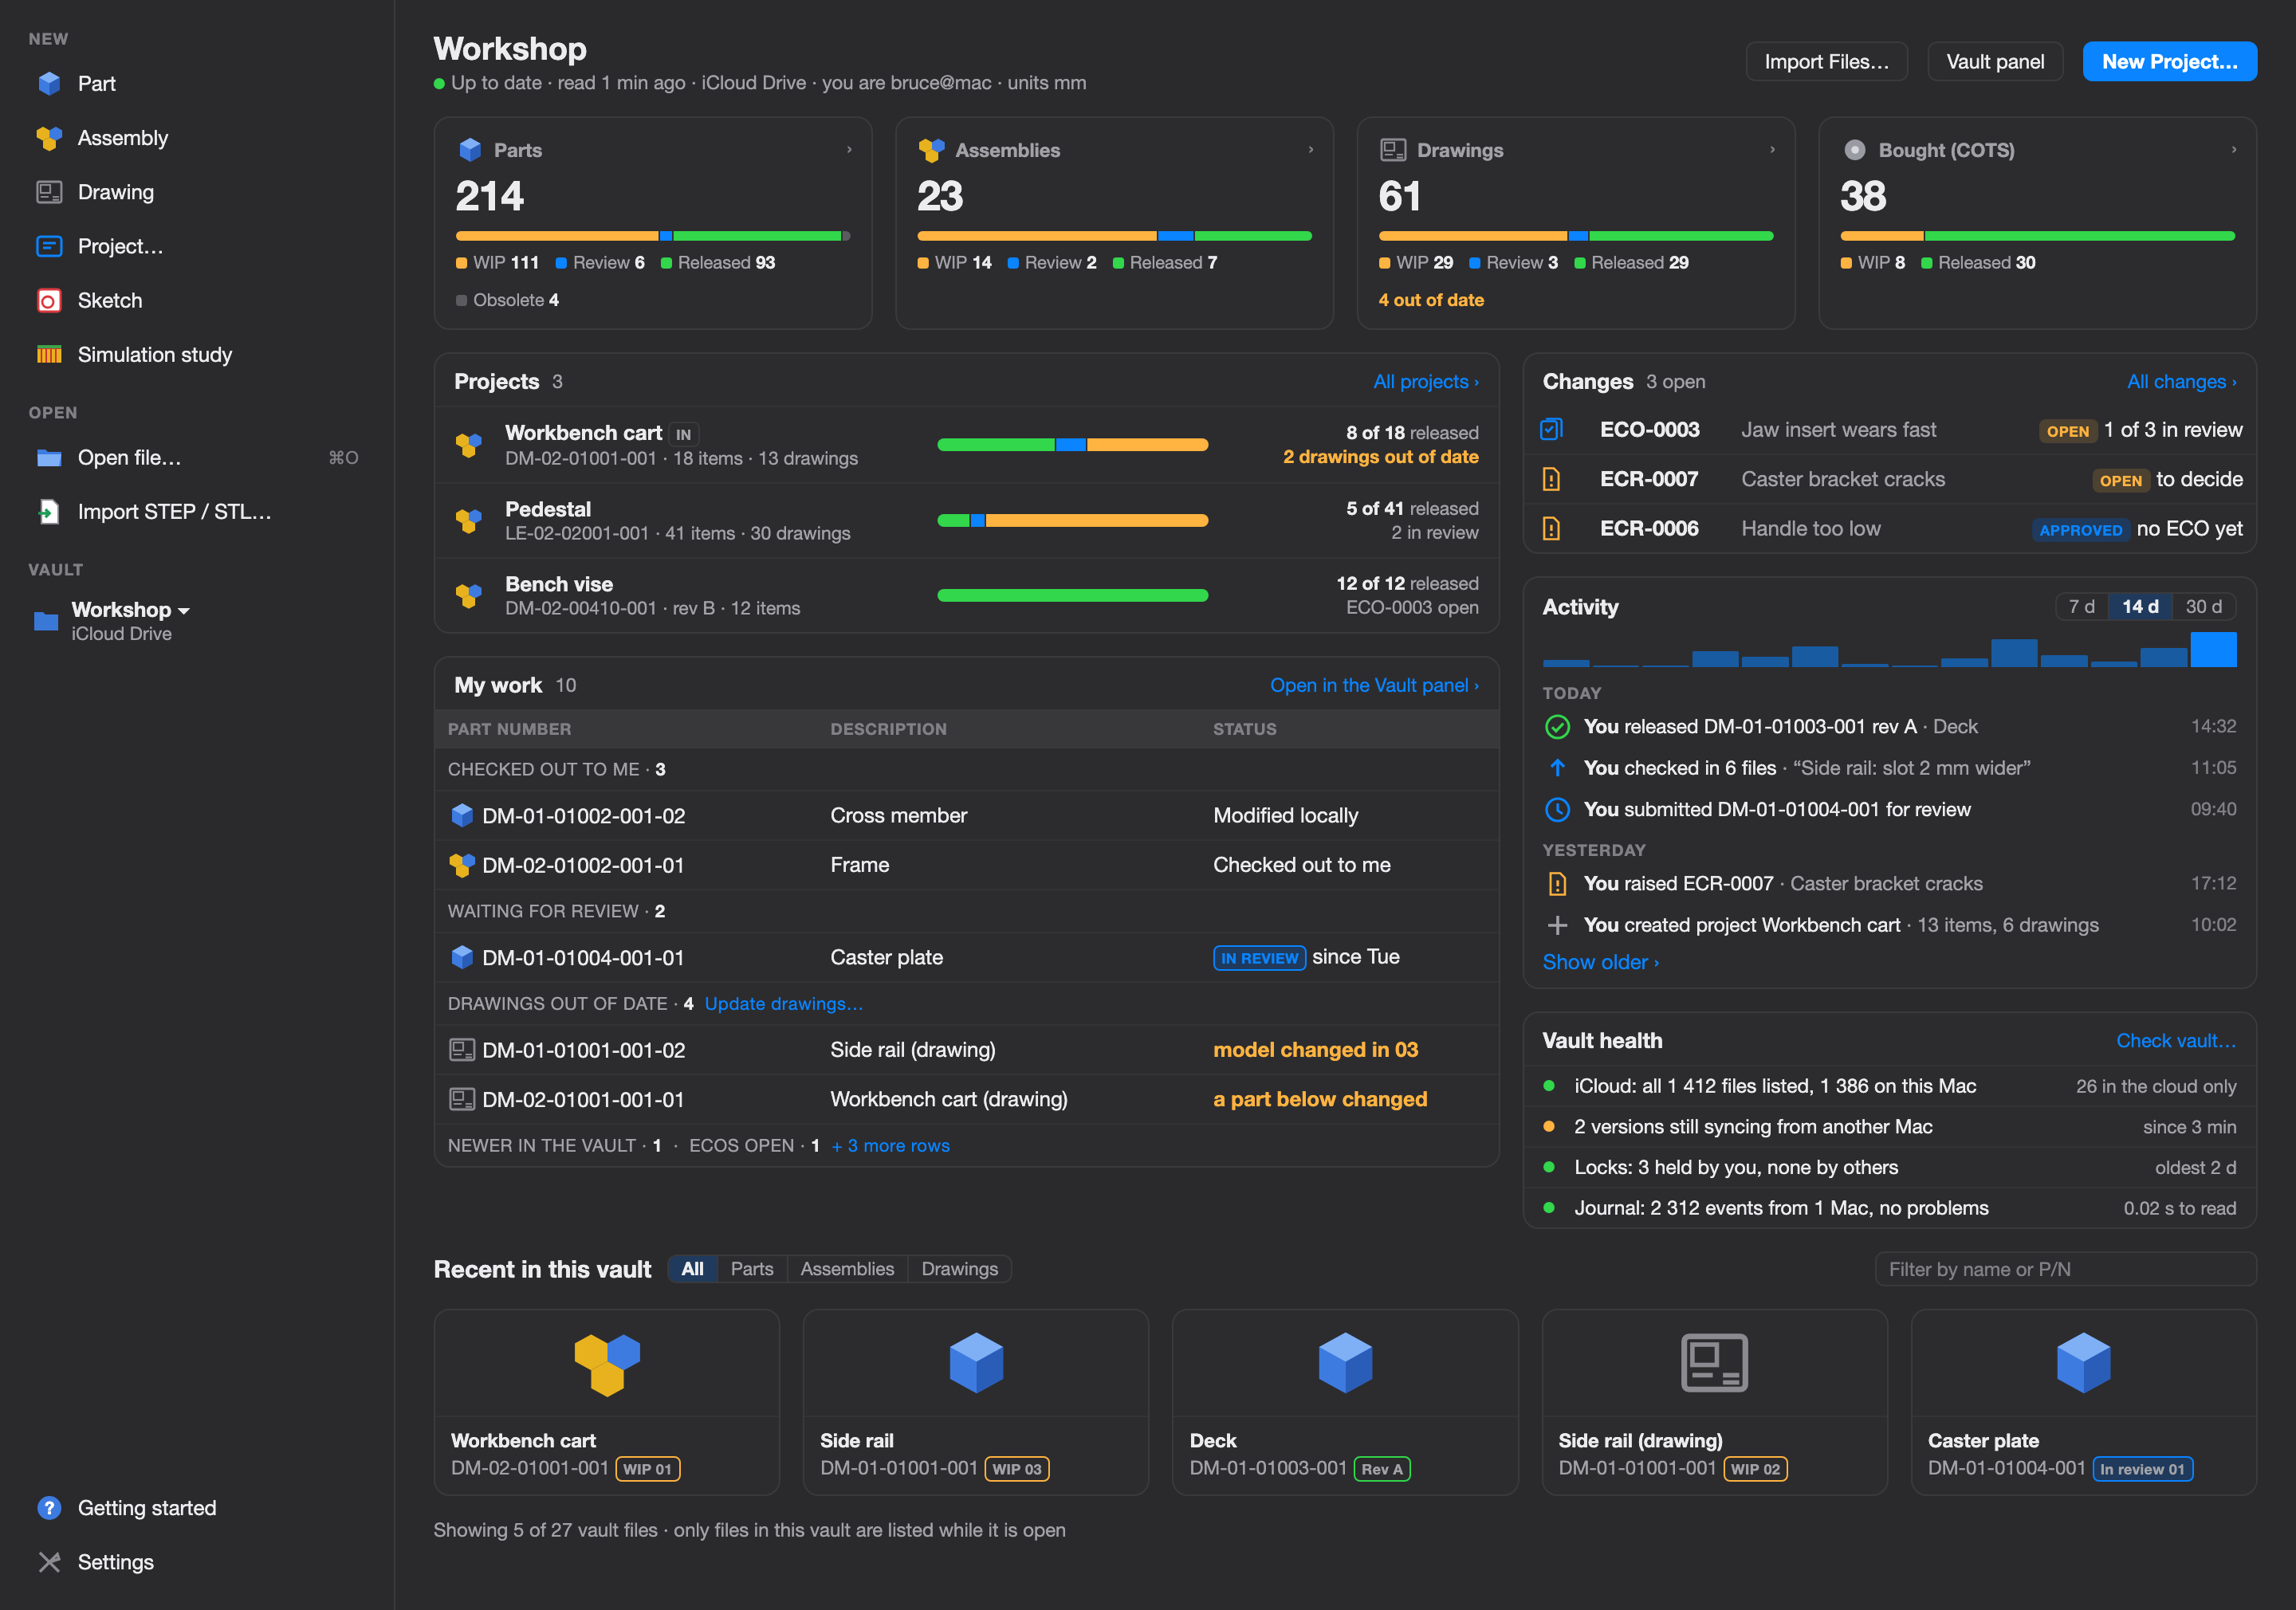
\includegraphics[width=\linewidth]{fig/pdm10_dashboard_dark.png}
\caption{The same page in dark mode: the theme's tokens (\file{BruceWorx Dark.yaml}), with the state colours of the badges and the Vault
panel's chips.}
\label{fig:pdm10-dark}
\end{figure}

\paragraph{Where it lives.} The dashboard is the Start page whenever a vault is open. The Start page already makes the vault
its home: the switcher, \emph{My work}, and recent files kept to the vault folder. With no vault open, the page stays as it
is today, with the recent files on this Mac. That is the only place local files appear (question~2). No new window and no
new tab is added: the Start tab is always first and pinned. A \emph{Dashboard} entry in the vault switcher's menu and the
Vault panel's header brings it forward.

\paragraph{Sections and where a click goes.}
\begin{center}
\small
\begin{tabularx}{\linewidth}{@{}>{\raggedright\arraybackslash}p{2.6cm}>{\raggedright\arraybackslash}p{4.6cm}X@{}}
\toprule
Section & Data (engine) & Click opens\\
\midrule
Tiles & items by type $\times$ state (\code{status()}); drawings out of date (PDM-09 \code{made\_from}) & Vault panel, chip
  \emph{Parts} etc.; a legend segment adds \code{state:wip}; ``out of date'' opens the Structure view's filter\\
Projects & PDM-09 project records, else top assemblies; roll-up as above & the Vault tab's Structure rooted at the top
  (PDM-09 step 5); until then, the Vault panel searching that P/N\\
My work & \code{Workspace.my\_work()} read-only, \code{my\_work\_rows}, drawings out of date; 3 rows per queue & a row opens
  the file (as today); ``$n$ more'' opens the Vault panel on that queue\\
Changes & \code{FolderVault.changes()}: open ECRs, approved ECRs without an ECO, open ECOs with what is pending & Vault
  panel, chip \emph{Changes}, that change selected\\
Activity & sorted events, folded; 7/14/30 days; \emph{Show older} pages back 50 & the item or change in the Vault panel
  (\code{show\_in\_panel})\\
Vault health & see below & \emph{Check vault\ldots}: a task panel listing each problem with its fix\\
Recent in this vault & the recent-files list kept to the vault folder (built) & the file\\
\bottomrule
\end{tabularx}
\end{center}

\paragraph{Vault health, line by line.}
\begin{itemize}[nosep]
  \item \textbf{iCloud}: objects the journal names that are on this Mac, in the cloud only (dataless, or a stand-in, via
        \code{needs\_download}; fine, they download on open), and \emph{still syncing}: named but not here at all. That is
        a version another Mac checked in whose file has not arrived. Orange after 10 minutes. Storage name from
        \code{storage\_name}.
  \item \textbf{Locks}: held by you and by others, with the oldest's age (needs the lock time, step~1). A lock older than
        14 days is flagged in \emph{Check vault\ldots}, with \emph{Break lock} (exists in the vault client).
  \item \textbf{Journal}: events, devices (journal files), problems from the replay (\code{FolderVault.problems}), conflict
        copies merged (e.g.\ \file{bruce@mac 2.jsonl}; harmless, listed), events dated in the future (a Mac with a wrong
        clock breaks the ordering), and the reading time.
\end{itemize}

\paragraph{An empty vault.} A new vault has no items, so tiles of zeros would say nothing. Until the first item exists, the
page shows a \emph{Get started} list instead (figure~\ref{fig:pdm10-empty}). Its first line, \emph{Vault settings}, is
ticked from the Create Vault answers. The next three are \emph{New Project\ldots}, \emph{Import Files\ldots} and
\emph{New Part}. The activity feed starts with ``You created the vault'', taken from the ref file's \code{created} field.
The tiles appear once the first item is checked in, and the list goes away.

\begin{figure}[!htbp]
\centering
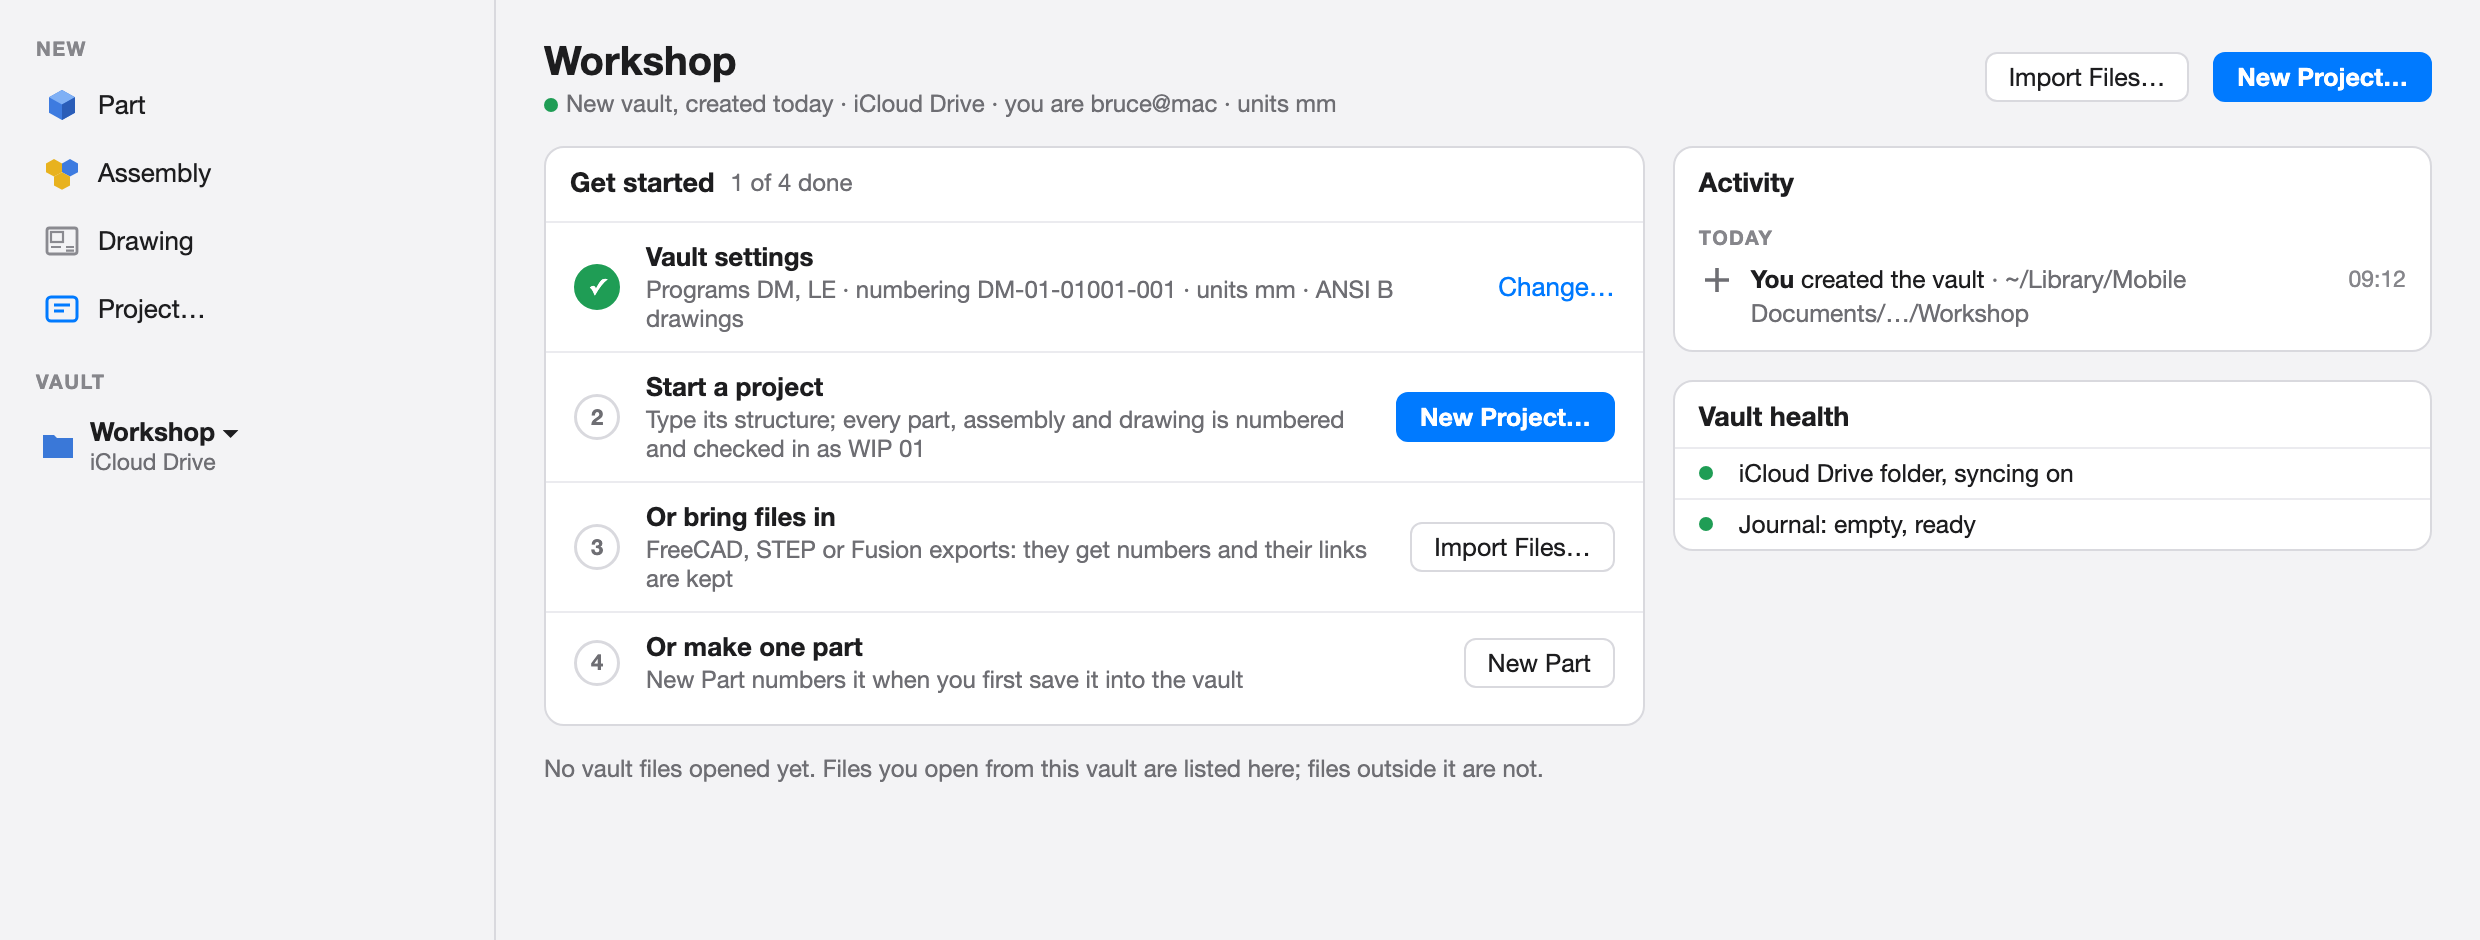
\includegraphics[width=0.86\linewidth]{fig/pdm10_dashboard_empty.png}
\caption{Mock: the first screen of a new, empty vault: what to do next instead of empty tiles.}
\label{fig:pdm10-empty}
\end{figure}

\paragraph{Refresh.} The page reads on the worker thread (\code{\_Loader}) when it is shown, after any vault operation in this
FreeCAD (the vault's listeners), and every 5\,s while it is visible: a signature check, then the tail or a full replay. The
last snapshot stays on screen while a new one is read, so the page never goes blank. The header's dot is green when the
snapshot is current and orange while files are still syncing. The worker opens the workspace \emph{read-only}, and the page
writes nothing.

\paragraph{Whose work is shown.} Everything in the vault is visible to anyone who can open the folder: the folder vault has
no permissions, so the dashboard hides nothing. \emph{My} means the actor pinned for this vault. Others' work shows as locks
(``checked out by alex'') and in the feed by name, with ``you'' for yours. A person with two Macs has two actors
(\code{bruce@mac}, \code{bruce@mbp}); question~4 decides whether they count as one.

%----------------------------------------------------------------------
\subsubsection*{4. Build order and effort}

\begin{center}
\small
\begin{tabularx}{\linewidth}{@{}lXl@{}}
\toprule
\# & Step & Effort\\
\midrule
1 & Engine: cycle check once after the replay and a cached BOM map (linear replay); the vault keeps its sorted events (no second
  read); lock start time; health counts with \code{needs\_download}; a read-only \code{Workspace}; contract tests unchanged
  and passing & 1\,d\\
2 & Incremental refresh: byte offsets per journal file, apply when every new event sorts after the last, else a full replay;
  tests for a late line from another Mac, a conflict copy, a half-synced line & 1\,d\\
3 & \file{bruceworx/vault\_dashboard.py} (FreeCAD-free): counts, queues, project roll-up, folded activity, changes,
  health, as one snapshot dict; the spike's generator becomes a test fixture (500 and 5\,000 items) with a time budget & 1.5\,d\\
4 & Start page: the dashboard layout when a vault is open (header, tiles, projects, capped \emph{My work}, changes,
  activity, health, recent vault files), \emph{Get started} for an empty vault, QSS blocks for light and dark & 2\,d\\
5 & Click-through: the Vault panel's search takes \code{state:}, \code{type:}, \code{lock:} and \code{change:} words; a
  \code{show\_filtered()} entry point; the \emph{Check vault\ldots} task panel & 1\,d\\
6 & Refresh: 5\,s signature poll while visible, vault listeners, last snapshot kept on screen & 0.5\,d\\
7 & Preference \code{BruceWorx/VaultDashboard} (on), pack and its test; acceptance on the scratch vaults, then on yours
  read-only; screenshots light and dark & 0.5\,d\\
\midrule
 & Total & 7.5\,d\\
\bottomrule
\end{tabularx}
\end{center}
Steps 1--3 stand alone and help every vault reader (Vault panel, CLI). Step~4 works before \eref{PDM-09}: its Projects
section shows top assemblies, and ``drawings out of date'' appears once PDM-09 records \code{made\_from}. Rows open the
Vault panel now and the Vault tab once \eref{UIX-12} has it. \emph{Acceptance:} on the 500-item scratch vault the page
fills in under 0.1\,s after the Start tab is shown. A check-in in this FreeCAD shows in the feed and the counts within 5\,s.
Every tile opens a list with exactly the count the tile shows. No file outside the vault appears while it is open.

\paragraph{Risks.} \emph{Stale numbers across Macs}: iCloud may deliver another Mac's journal minutes late. The header says when
the page was read, ``still syncing'' says what has not arrived, and a late line triggers a full replay. \emph{Wrong
clocks}: the journal is ordered by time, so a Mac whose clock is off reorders events. Health flags future dates; the cure
(a Lamport counter in the event) is a contract change and stays out of scope. \emph{Engine change}: moving the cycle check
alters the replay. The contract tests and a byte-for-byte comparison of \code{status()} before and after, on the scratch
vaults, guard it. \emph{Python on the main thread} gets less time during a long replay (up to 28\,ms pauses at 5\,000
items). That is invisible at your size and shrinks with step~1. \emph{Too much on one page}: the sections are capped, and
each can be folded (remembered per vault).

%----------------------------------------------------------------------
\paragraph{Your answers (24 Oct).} Recommendations for 1 and 3--9. \textbf{2} changed: files outside the vault
do not appear on the dashboard, but the Start page gets a \emph{Recent files} tab beside it (the vault dashboard and the
local recent files are two tabs of the Start page; the dashboard is the default while a vault is open, Recent files
when none is). Building started 24 Oct.

\subsubsection*{Questions before PDM-10 starts}

\begin{enumerate}
  \item \textbf{Where the dashboard lives.} The Start page when a vault is open (figure~\ref{fig:pdm10-light}), or a separate
        \emph{Vault} tab beside it?\\
        \emph{Recommendation:} the Start page. It is already the vault's home (switcher, \emph{My work}, vault-only recent
        files), it is always the first tab, and a second home would split them.
  \item \textbf{Local files while a vault is open.} Should files outside the vault appear anywhere on the page?\\
        \emph{Recommendation:} no, as you said. They stay in \emph{File $\rightarrow$ Open Recent} (FreeCAD's menu, unchanged)
        and come back on the Start page when you close the vault. No ``files outside the vault'' link.
  \item \textbf{The first screen of an empty vault.} The \emph{Get started} list (figure~\ref{fig:pdm10-empty}), or empty tiles?\\
        \emph{Recommendation:} the list. It disappears for good once the first item is checked in.
  \item \textbf{Who is ``me''.} Today \emph{my} work means one actor, \code{user@mac}. When you use a second Mac, should
        \code{bruce@mac} and \code{bruce@mbp} count as one person on the dashboard?\\
        \emph{Recommendation:} yes, by the part before the @. Locks stay per Mac, because a file checked out on the iMac
        is still not writable on the laptop. The queue then says ``checked out to you on iMac''.
  \item \textbf{Other people's work, later.} With more users, should the dashboard show everyone's locks and activity, or only
        yours unless asked?\\
        \emph{Recommendation:} everyone's. The folder vault has no permissions, so hiding would only be cosmetic, and in a
        small team seeing who holds what is the point. The feed gets a \emph{Mine / Everyone} switch (default Everyone).
  \item \textbf{Activity range.} How far back should the feed go by default?\\
        \emph{Recommendation:} 14 days, with 7/14/30 to switch and \emph{Show older}. Check-outs are hidden unless
        \emph{Show all} is on.
  \item \textbf{Projects before PDM-09.} Until projects are records, should the Projects section show top assemblies, or stay
        hidden?\\
        \emph{Recommendation:} show top assemblies, labelled so. Hide the section when there are more than 12, because
        then the BOMs are not recorded yet and the list would mislead.
  \item \textbf{The engine change.} May step~1 change the replay in \file{pdm\_folder.py}/\file{pdm.py} (cycle check once,
        cached BOM map)? It is \eref{PDM-06}'s code.\\
        \emph{Recommendation:} yes, in step~1, guarded by the contract tests and a \code{status()} comparison on the
        scratch vaults. It speeds up every reader, not only the dashboard.
  \item \textbf{Old locks.} Should a lock older than some age be flagged, and after how long?\\
        \emph{Recommendation:} 14 days, as a health line and in \emph{Check vault\ldots} with \emph{Break lock}. Never
        break a lock automatically.
\end{enumerate}

%----------------------------------------------------------------------
\subsubsection*{Built (24 Oct 2026)}\label{sec:pdm10-built}

\paragraph{Your answer (24 Oct, evening).} The \emph{Recent files} tab keeps every recent file on this Mac, the open vault's files included (as built).


Steps 1 to 7 were built in the plan's order, with your answers: recommendations for questions 1 and 3--9, and for
question~2 the Start page's two tabs. Your vault \emph{Vector} was never opened: every run used scratch vaults made
by the engine and a config copy whose \code{VaultPath} points at them.

\begin{itemize}[nosep]
  \item \textbf{Linear replay} (step 1, \file{pdm.py}, \file{pdm\_folder.py}). \code{set\_bom} checks the whole BOM
        graph for a cycle only when it records a line (\code{strict}); a replay checks once at the end
        (\code{Vault.find\_cycle}) and lists a cycle that two Macs' journals made as a problem. A cached BOM map was
        not needed: with the check out of the replay nothing rebuilds the map while replaying. Every reader of
        \code{status()}, BOMs, changes, locks, versions and revision records was compared byte for byte before and
        after on the 500, 2\,000 and 5\,000-item scratch vaults: identical. Open the vault (read and replay):
        9 / 74 / 420\,ms before, \textbf{6 / 21 / 59\,ms} after.
  \item \textbf{What the page needs from the engine.} The vault keeps the sorted events it read (\code{events}; the
        Start page no longer reads the journal twice), keeps when each lock was taken (\code{lock\_times}), and
        \code{object\_health()} counts objects on this Mac, in iCloud only (dataless or a \file{.icloud} stand-in) and
        still syncing. \code{missing\_objects()} no longer counts a stand-in as missing; \emph{Move Vault} still waits
        for stand-ins, since a stand-in cannot be copied.
  \item \textbf{The \file{state.json} race} is gone: \code{Workspace(vault, read\_only=True)} never saves, and its
        operations refuse to run. The Start page's worker uses only that.
  \item \textbf{Reading only what is new} (step 2, \code{FolderVault.update}). Byte offsets per journal file; new
        complete lines that all sort after the last event are applied in place; a late line, a clock behind, a file
        that shrank, was replaced or went away replays everything. A half-synced line waits for its end; a conflict
        copy whose events are known changes nothing.
  \item \textbf{\file{bruceworx/vault\_dashboard.py}} (step 3, FreeCAD-free): the snapshot of section~2: tiles, top
        assemblies with a memoised roll-up (each item once, plus drawings; hidden above 12), My work (3 rows a queue;
        \code{bruce@mbp} counts as you, ``checked out to you on mbp''), changes and what each waits for, the folded
        feed (10\,min runs, 14 days, check-outs and BOM records only with \emph{Show check-outs}, \emph{Only mine}),
        health. The spike's generator is the test fixture \file{tests/vault\_fixture.py}; on its 500-item vault the
        page's data takes about 25\,ms to read and build (test budget 0.1\,s).
  \item \textbf{The Start page} (steps 4 and 6, \file{bruceworx\_start.py}, new \file{bruceworx\_dashboard.py}). Two
        tabs: \emph{Vault dashboard} (the default while a vault is open) and \emph{Recent files} (every recent file on
        this Mac; the default with no vault). The dashboard keeps to the vault: its \emph{Recent in this vault} uses the
        \code{vault\_folder}/\code{in\_folder} rule. The worker keeps one \code{FolderVault} and reads new lines only;
        the page looks every 5\,s while visible and at once after a vault operation in this FreeCAD (a check-in showed
        in the feed 0.12\,s later). The last snapshot stays on screen while a new one is read. Light and dark come
        from the theme tokens (figure~\ref{fig:pdm10-built}); an empty vault shows \emph{Get started}
        (figure~\ref{fig:pdm10-built-empty}).
  \item \textbf{Click-through} (step 5). The Vault panel's search takes \code{type:}, \code{state:}, \code{lock:},
        \code{status:} and \code{change:} words, and \code{show\_filtered()} opens it on a chip and words. Every tile
        opened a list with exactly its count (340 / 55 / 85 / 20 on the scratch vault), the legend entries add the
        state, \emph{+ 22 more} opens the queue, rows select their item or change. \emph{Check vault\ldots} is a task
        panel listing each problem with its fix (\emph{Break Lock\ldots} for a lock older than 14 days). The vault
        switcher's menu and the Vault panel's menu have \emph{Dashboard}.
  \item \textbf{Preference} (step 7): Preferences $\rightarrow$ BruceWorx $\rightarrow$ \emph{Vault dashboard on the
        Start page} (\code{BruceWorx/VaultDashboard}, on). Off keeps the page as it was.
  \item \textbf{Not yet:} \emph{New Project\ldots} is shown greyed until PDM-09 adds its command; ``drawings out of
        date'' waits for PDM-09's \code{made\_from}; sections cannot be folded yet.
  \item \textbf{Tests.} Add-on: \file{test\_pdm\_replay.py} (linear replay, lock times, stand-ins, read-only
        workspace, incremental reading) and \file{test\_vault\_dashboard.py}; all 423 add-on tests pass. FreeCAD:
        \code{TestBruceWorxStart} (tabs, header, query words), \code{TestBruceWorxChanges}, \code{TestBruceWorxBom},
        \code{TestBruceWorx}, \code{TestBruceWorxPattern}, \code{TestAssemblyWorkbench} pass.
\end{itemize}

\begin{figure}[!htbp]
\centering
\IfFileExists{fig/pdm10_built_light.png}{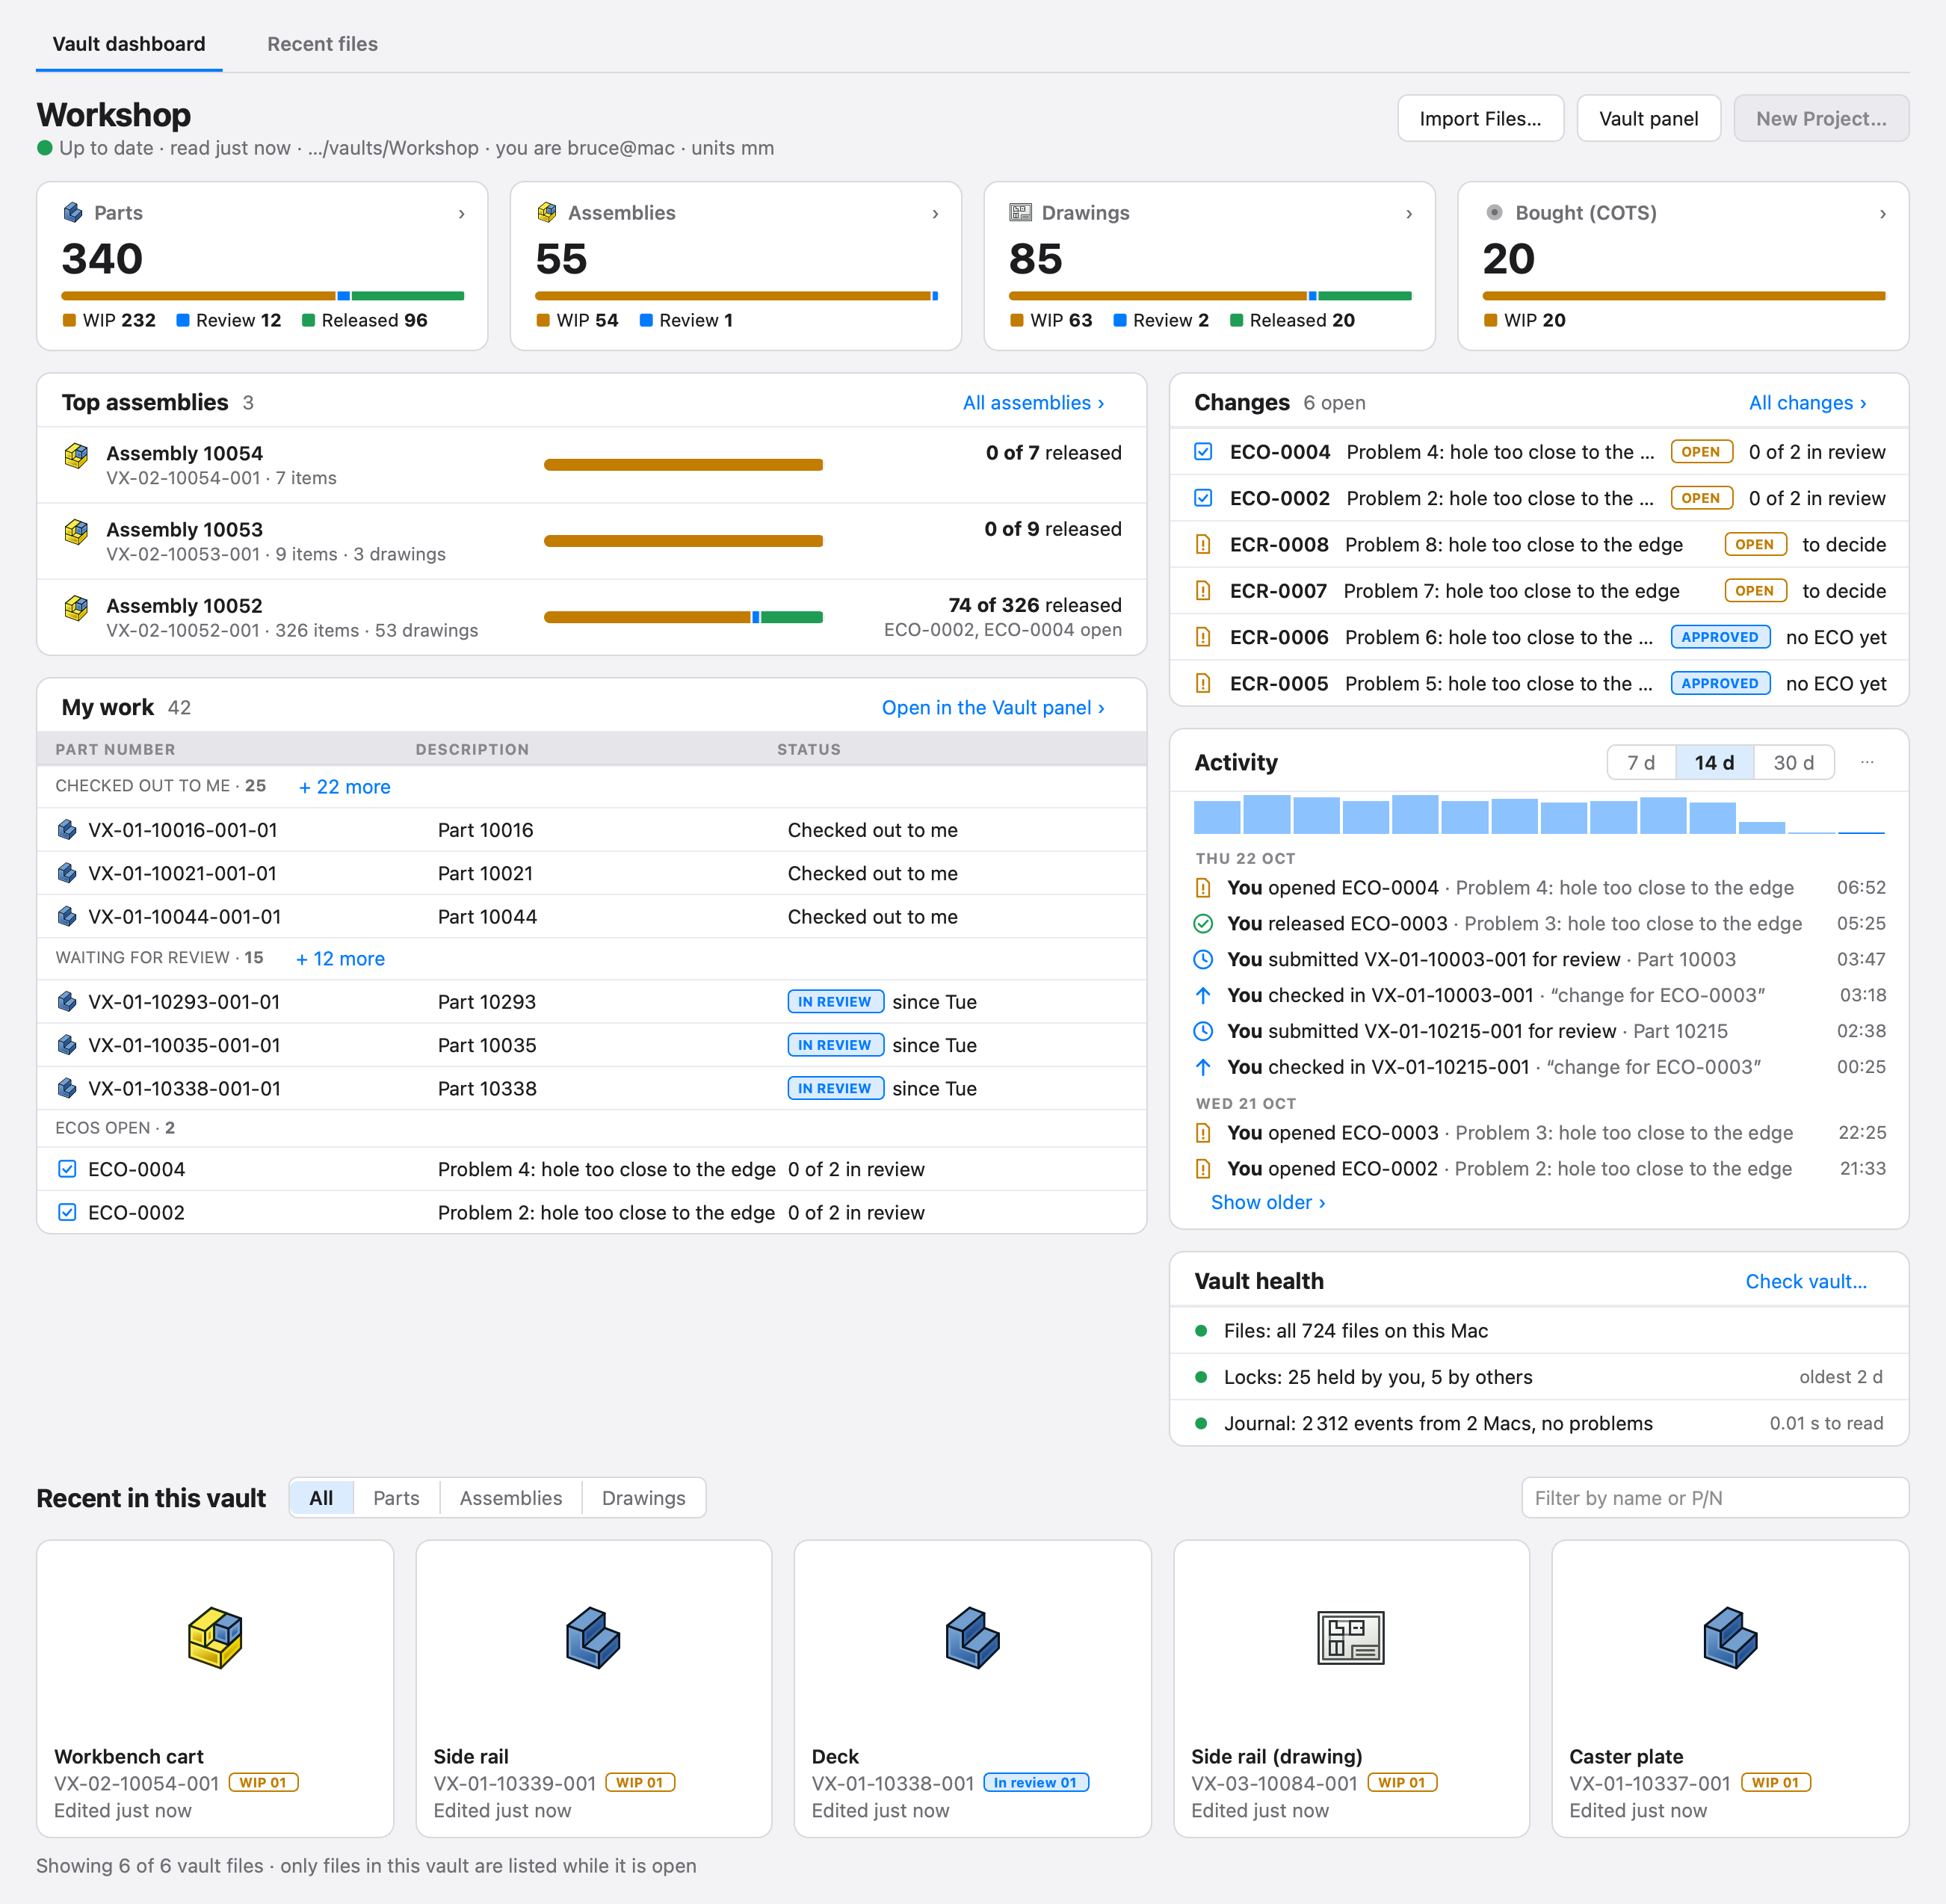
\includegraphics[width=0.49\linewidth]{fig/pdm10_built_light.png}}{\fbox{pdm10\_built\_light.png}}\hfill
\IfFileExists{fig/pdm10_built_dark.png}{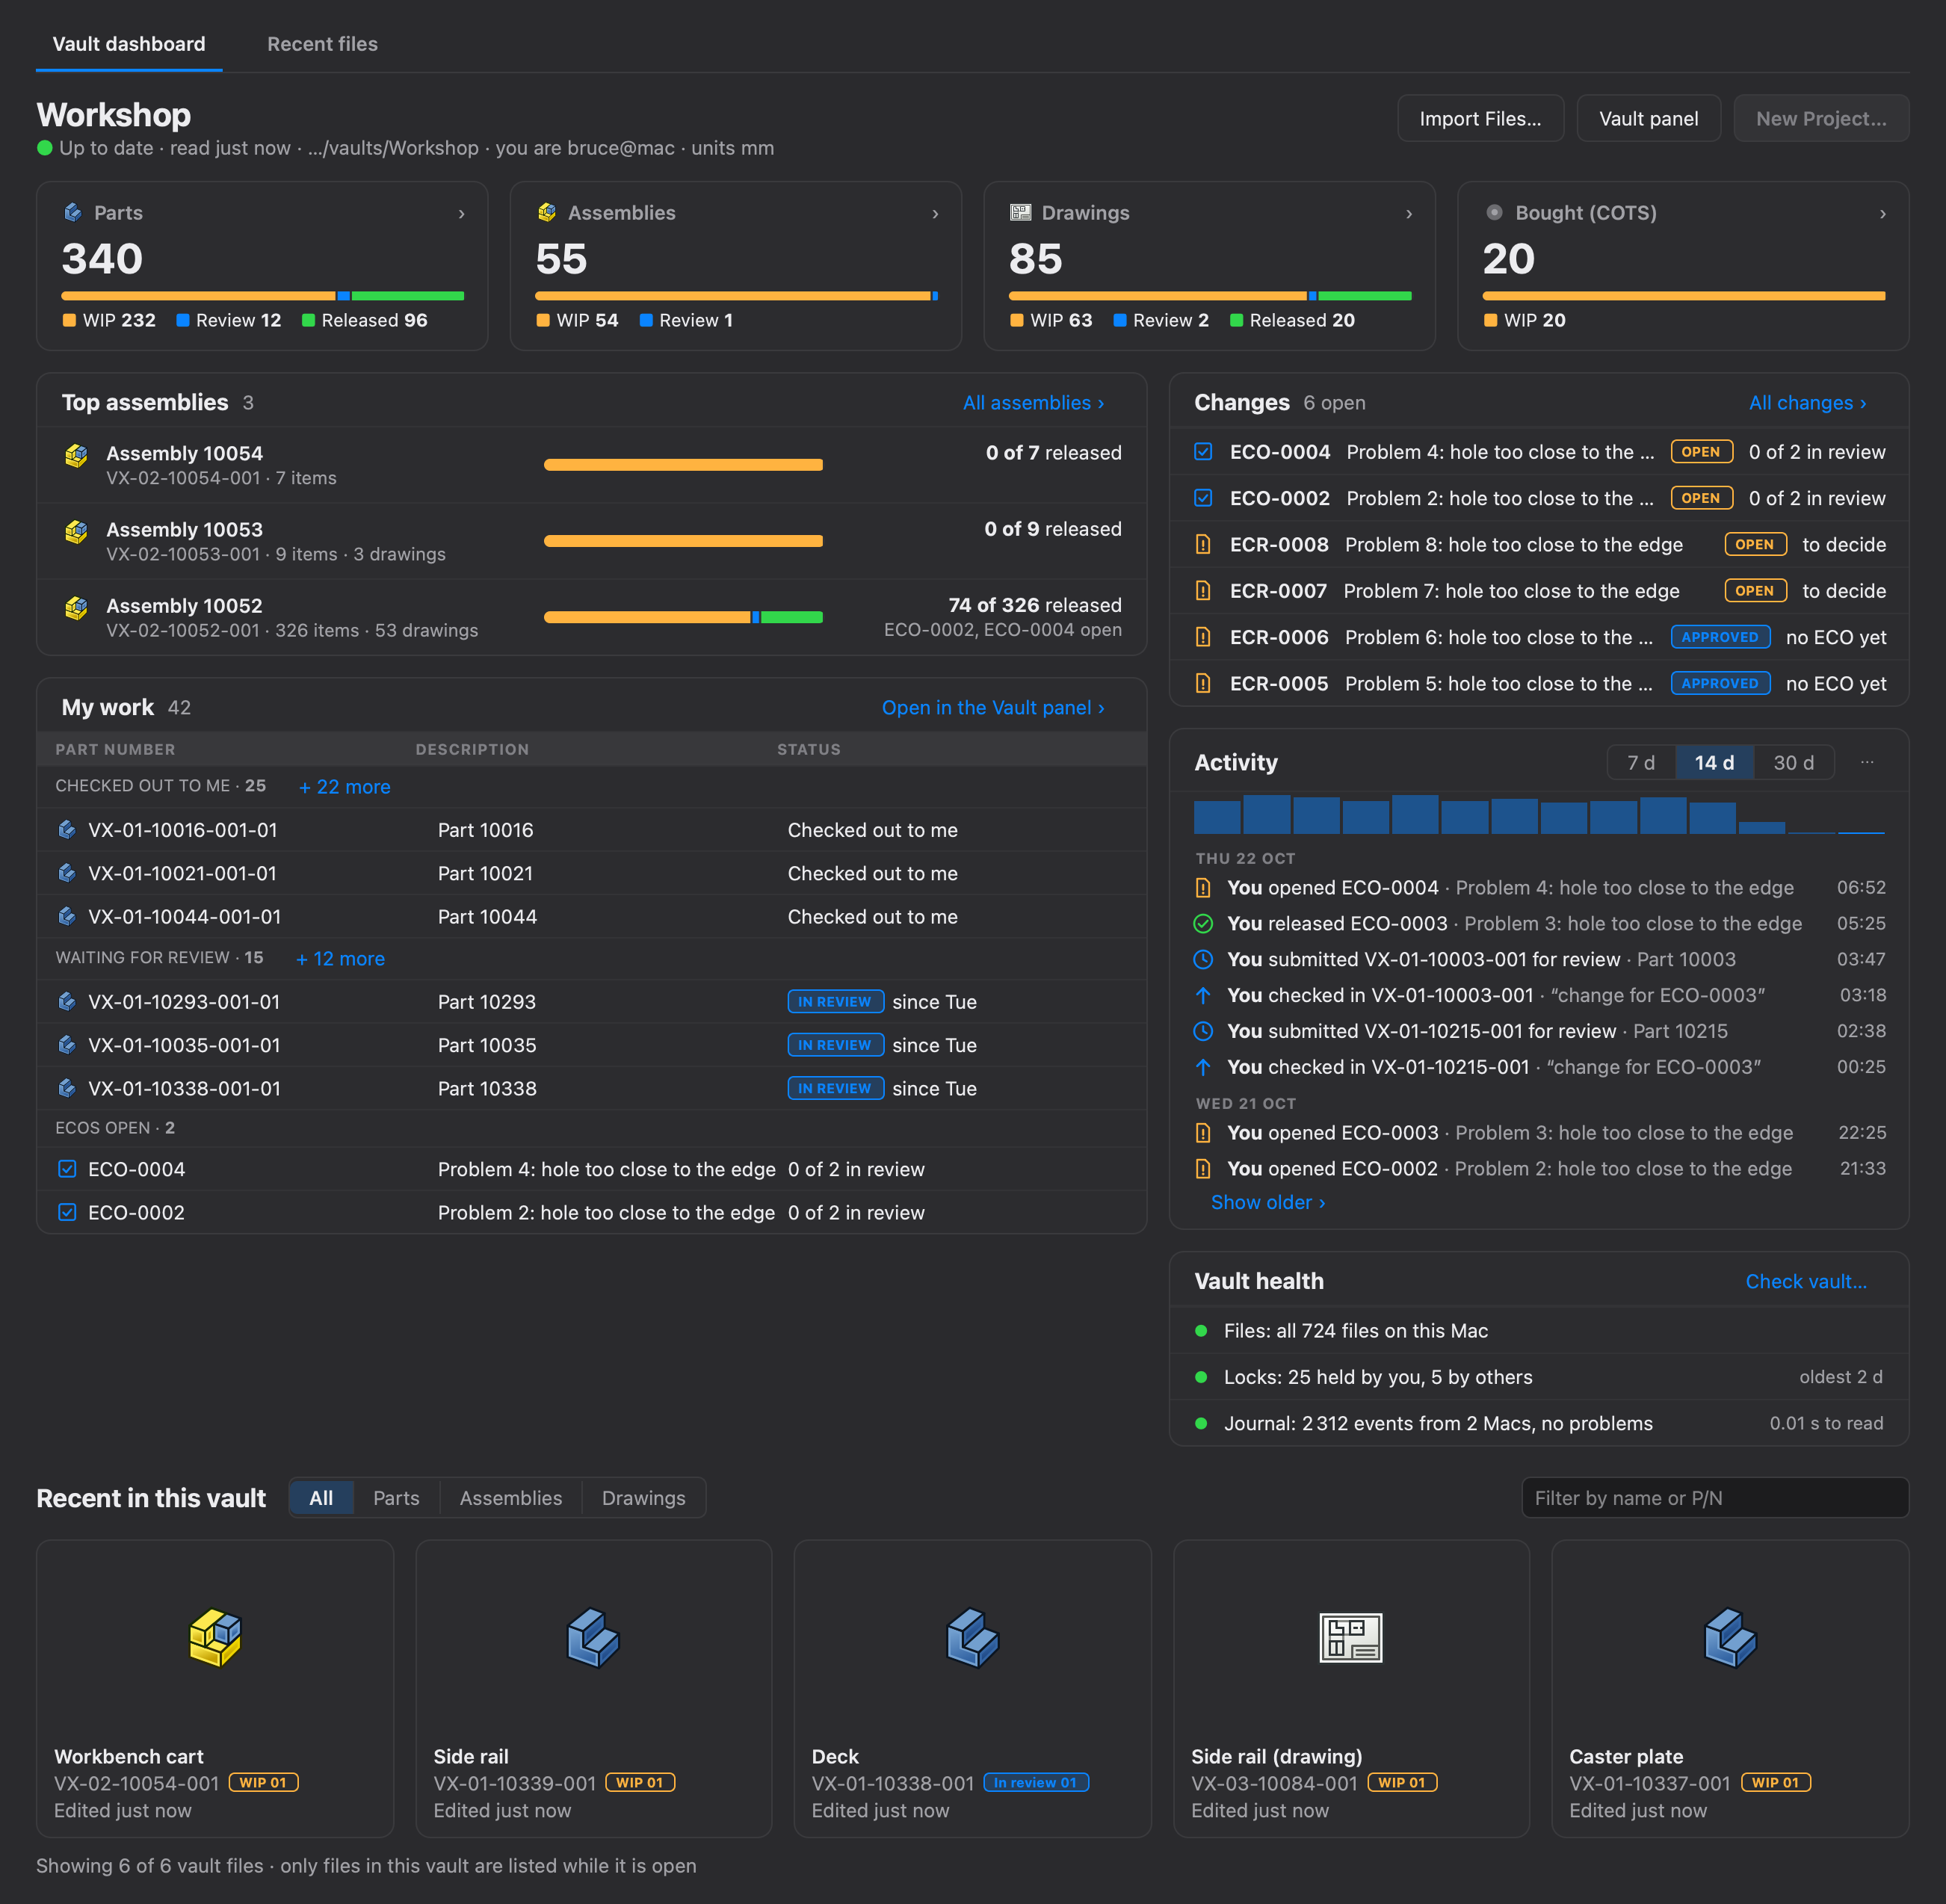
\includegraphics[width=0.49\linewidth]{fig/pdm10_built_dark.png}}{\fbox{pdm10\_built\_dark.png}}
\caption{As built: the dashboard of the 500-item scratch vault, light and dark (the page's main area; the Start page's
left column is unchanged). Compare figures~\ref{fig:pdm10-light} and~\ref{fig:pdm10-dark}.}
\label{fig:pdm10-built}
\end{figure}

\begin{figure}[!htbp]
\centering
\IfFileExists{fig/pdm10_built_empty.png}{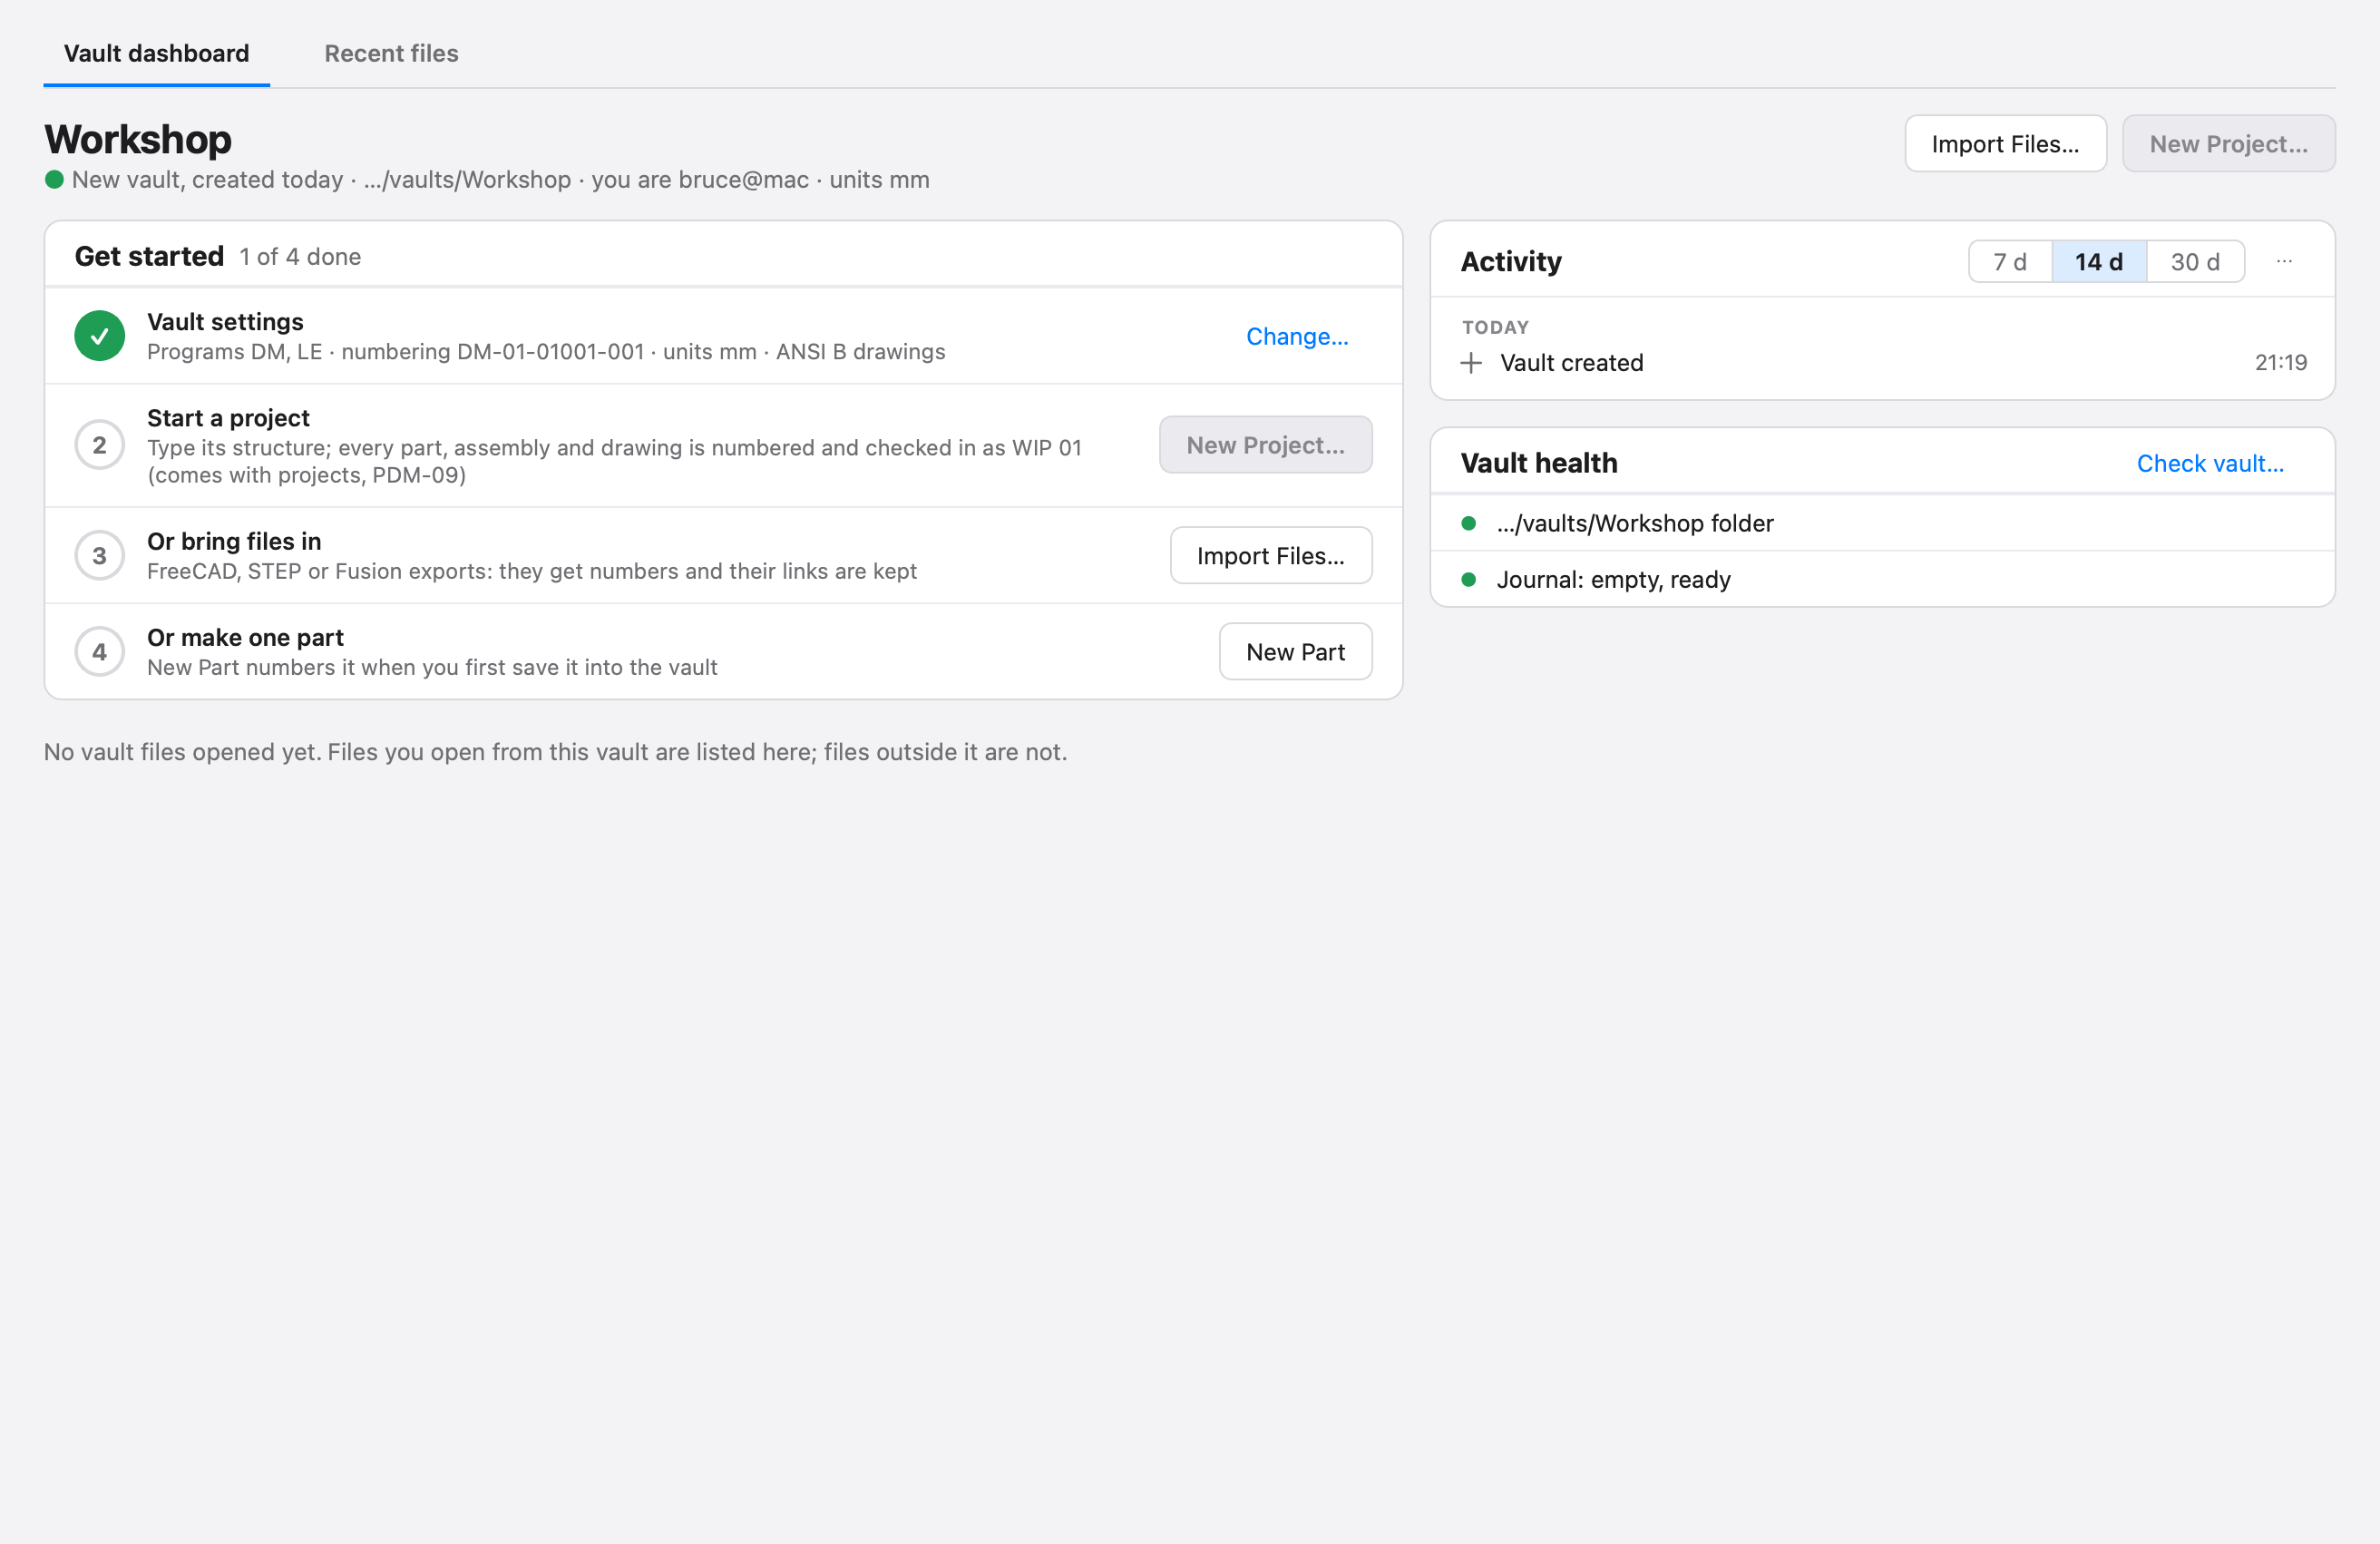
\includegraphics[width=0.8\linewidth]{fig/pdm10_built_empty.png}}{\fbox{pdm10\_built\_empty.png}}
\caption{As built: a new, empty vault made with the Create Vault engine (compare figure~\ref{fig:pdm10-empty}).}
\label{fig:pdm10-built-empty}
\end{figure}

\paragraph{Acceptance (done 25 Oct).} Checked in the GUI on a 60-item fixture vault: each of the four tiles and eight
state entries opens the Files tab with exactly its count (for example \emph{Parts} 42 and \emph{WIP parts} 30 give
``42 items of 60'' and ``30 items of 60''); a check-in written to the journal by another Mac (\code{other@mac2}) shows
in the tiles and the activity feed after 0.8\,s, inside the 5\,s budget; the 500-item read stays under 0.1\,s
(\file{test\_vault\_dashboard.py}). The tiles' tool tips now name the Files tab and keep WIP and COTS in capitals.
